\documentclass[11pt,twoside,a4paper]{book}

\usepackage[czech, english]{babel}
 \usepackage[OT1]{fontenc} % pouzije EC fonty
\usepackage[utf8]{inputenc}
\usepackage{lmodern}
\usepackage{graphicx}

\usepackage{mathtools}
\usepackage{indentfirst} %1. odstavec jako v cestine.
\usepackage{k336_thesis_macros} 
\usepackage{hyperref}
\hypersetup{
    bookmarks=true,         % show bookmarks bar?
    unicode=true,			% non-Latin characters in Acrobat’s bookmark
    colorlinks=true,       	% false: boxed links; true: colored links
    linkcolor=blue,			% color of internal links (change box color with linkbordercolor)
    citecolor=blue,        	% color of links to bibliography
}

\usepackage[square, numbers]{natbib}             % sazba pouzite literatury


\newcommand\Department{Katedra počítačů}
\newcommand\Faculty{Fakulta elektrotechnická}
\newcommand\University{České vysoké učení technické v Praze}
\newcommand\labelSupervisor{Vedoucí práce}
\newcommand\labelStudProgram{Studijní program}
\newcommand\labelStudBranch{Obor}

\newcommand\TypeOfWork{Diplomová práce} \typeout{Diplomova prace}
\newcommand\StudProgram{Otevřená informatika, Magisterský}
\newcommand\StudBranch{Softwarové inženýrství}

\newcommand\WorkTitle{Pohledově závislá aplikace textur v reálném čase}
\newcommand\FirstandFamilyName{Bc. Daniel Princ} \newcommand\Supervisor{Ing.
David Sedláček, Ph.D.}


\let\oldUrl\url \renewcommand\url[1]{<\texttt{\oldUrl{#1}}>}


\begin{document}
\selectlanguage{czech} 

\coverpagestarts

\acknowledgements \noindent \noindent Chtěl bych poděkovat vedoucímu této práce,
panu Ing. Davidovi Sedláčkovi, Ph.D., za poskytnutí cenných rad a nápadů.

\declaration{V~Praze,  12. 5. 2014}
 
\abstractpage
TBD

\vglue60mm

\tableofcontents

\listoffigures

\listoftables

\mainbodystarts
% horizontalní mezera mezi dvema odstavci \parskip=5pt 11.12.2008 parskip +
% tolerance
\normalfont \parskip=0.2\baselineskip plus 0.2\baselineskip minus
0.1\baselineskip


\chapter{Úvod}
V dnešní době umožňuje počítačová grafika renderovat realistické obrazy 3D
světa. Nicméně aby toto bylo možné, musí existovat 3D modely objektů, které
chceme zobrazovat. Tradiční způsob, jak získat tyto modely, je jejich ruční
vytváření v modelovacích programech. To je velmi pracný a zdlouhavý proces
a~jeho výsledek není dostatečně realistický. Proto se v současnosti vyvíjí
postupy, jak přímo digitalizovat reálné objekty. Existují dva základní přístupy,
které se o toto pokoušejí. Nejpřesnější metoda je pravděpodobně laserové
skenování objektů. Druhou, mnohem levnější a dostupnější variantou, je rekonstrukce objektů z
fotografií. Těmito problémy se zabývá počítačové vidění a částečně také
počítačová grafika, do které spadá zobrazování rekonstruovaných modelů. Cílem 3D
počítačové rekonstrukce je tedy co nejvěrněji převést reálné objekty do
digitální podoby. Aplikaci najdeme ve virtuální realitě, online prohlídkách,
počítačových animacích nebo v herním či filmovém průmyslu.

Tato práce se zabývá jednou částí 3D rekonstrukce a to texturování objektů z
fotografií. Na vstupu očekáváme již zrekonstruovaný 3D model (síť trojúhelníků)
a větší množství (desítky až stovky) kalibrovaných fotografií z různých úhlů. Textura společně s materiálem slouží k popisu povrchu a je důležitá pro vnímání barvy a detailní struktury povrchu \cite{mpg}. Aplikace textury vede z výraznému zvýšení vizuální kvality objektu za relativně malou cenu.  Často je vizuálně i výkonově jednodušší použít detailní texturu a jednoduchý model s menším počtem vrcholů.

Syntéza textur z fotografií je poměrně složitá, protože 	na výsledný model se díváme i z jiných pohledů, než ze kterých byly pořízeny fotografie. Problémy, které při tomto procesu vznikají jsou popsány zejména v následující kapitole. Cílem této práce je vytvořit aplikaci, která v reálném čase mapuje fotografie na model. Protože aplikace funguje v reálném čase, může zohlednit aktuální pohled virtuální kamery a na základě pozice kamery vybrat nejvhodnější fotografie pro vytvoření textury. K tomu využívá velkého výkonu současných GPU.

[[obrázek model s a bez textur TODO]]


\chapter{Analýza problému a návrh řešení} %??

\section{Popis problému}

Předpokládejme, že se díváme na statickou scénu s konstantním osvětlením, kde se pohybuje pouze pozorovatel. Za těchto podmínek můžeme popsat libovolnou fotografii pomocí pozice a orientace kamery. Pokud bychom vyfotili sférickou fotografii v každé možné pozici kamery, mohli bychom vyrenderovat kompletní scénu z libovolného pohledu. Kombinací všech 3D pozic kamery $(x, y, z)$ a směrů $(\theta, \phi)$ získáme plenoptickou funkci $\textbf{L}(x, y, z, \theta, \phi)$ \cite{Adelson91}. Snahou je aproximovat funkci \textbf{L} pomocí konečného množství diskrétních vzorků $(x, y, z, \theta, \phi)$ a z této reprezentace efektivně renderovat nové pohledy (s pomocí 3D geometrie). Povrch geometrie můžeme popsat jako funkci $\textbf{G} : (x, y, z, \theta, \phi) \to (x_0, y_0, z_0)$, tedy jako mapování pohledových paprsků na 3D souřadnice povrchu. Jako $\textbf{G}_0$ si označíme funkci skutečného povrchu, $\textbf{G}_A$  reprezentuje aproximovaný povrch (rekonstruovaný 3D model), viz obr. \ref{fig:projection-error}.

\begin{figure}[hb]
\begin{center}
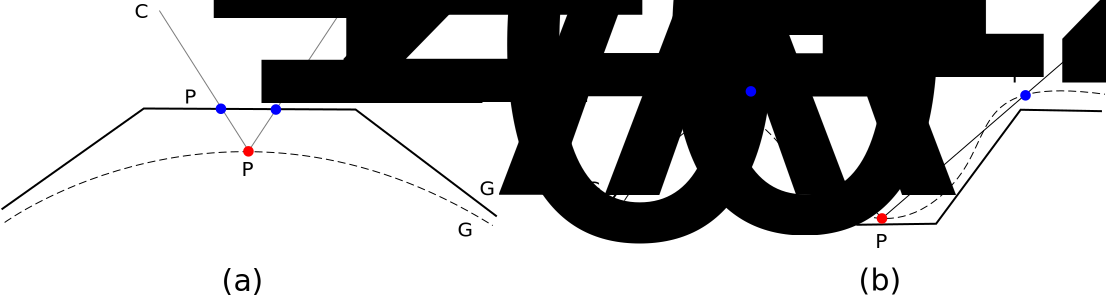
\includegraphics[width=\textwidth]{figures/projection-error}
\label{fig:projection-error}
\caption{(a) chyby v geometrii způsobují chybnou projekci, bod P na původní geometrii je promítnut na body $P_1$ a $P_2$ na aproximované geometrii. (b) chyby ve viditelnosti, bod P je chybně viditelný z kamery $C_2$ a naopak není viditelný z kamery $C_1$.}
\end{center}
\end{figure}

Důležitým prvkem je projekční matice kamery, která nám určuje projekční mapování 3D bodu $(x, y, z)$ do 2D souřadnic $(s, t)$ v $i$-té fotografii  $\textbf{P}_i: (x, y, z) \to (s, t)$, viz sekce \ref{sec:matice-kamery}.  Z promítnuté pozice v obrázku pak můžeme přiřadit 3D bodu barvu $\textbf{I}_i : (s, t) \to (r, g, b)$. Poté libovolný nový pohled $\textbf{I}^V$ z virtuální kamery $V$ můžeme vyjádřit pomocí rovnice \ref{eq:iview} \cite{floating-textures}.

\begin{align}
\label{eq:iview}
\textbf{I}^V(x, y, z, \theta, \phi) = \sum_{i} \textbf{I}_{i}^{V}(x, y, z, \theta, \phi)~\omega_i
\end{align}

\noindent kde

\begin{align}
\label{eq:linear-comb-plen}
\textbf{I}_{i}^{V}(x, y, z, \theta, \phi) &=\textbf{I}_{i}(\textbf{P}_{i}(\textbf{G}_A(x, y, z, \theta, \phi)))\\
\label{eq:linear-weighting}
 \omega_i &= \delta_i(\textbf{G}_A(x, y, z, \theta, \phi)) w_i(x, y, z, \theta, \phi)
\end{align}

\noindent a $\sum_i \omega_i = 1$. Notace $ \textbf{I}_{i}^{V}$ značí vyrenderovaný obrázek z pohledu $V$ promítnutím vstupní fotografie  $\textbf{I}_{i}$ jako textury na povrch  $\textbf{G}_A$. $\delta_i$ určuje viditelnost a je 1, pokud je bod na povrchu $\textbf{G}_A$ viditelný v kameře $i$ a 0 pokud není. $w_i$ je funkce, která určuje váhu kamery $i$ pro každý paprsek.

Zásadní problém spočívá v tom, že $\textbf{G}_A \neq \textbf{G}_0$, tedy již vstupní data vztahu \ref{eq:linear-comb-plen} jsou zatížena chybou (obr. \ref{fig:projection-error}). Problémy přináší také nepřesná kalibrace kamery $\textbf{P}_i$, což způsobuje další nepřesnosti při mapování.


\subsection{Matice kamery}
\label{sec:matice-kamery}

Nejběžněji se v počítačové grafice a vidění používá perspektivní projekce, která promítá 3D body $p$ na 2D body $x$ vydělením jejich $z$ souřadnicí \cite{Szeliski}. V homogeních souřadnicích má kanonická perspektivní matice \textbf{P}$_0$ jednoduchou formu:
\begin{align}
\label{eq:persp-projection}
x = 
\underbrace{
\begin{bmatrix}
1 & 0 & 0 & 0 \\
0 & 1 & 0 & 0 \\
0 & 0 & 1 & 0 \\
\end{bmatrix}}_\text{\textbf{P}$_0$}
p
\end{align}
\noindent

Po promítnutí 3D bodu projekční kamerou je nutné transformovat souřadnice na základě vlastností senzoru a orientace kamery vzhledem k počátku souřadnicového systému.  \emph{Kalibrační matice} \textbf{K} transformuje kanonickou perspektivní kameru na standardní projekční kameru \textbf{P}: 
\begin{align}
\label{eq:calibration-matrix}
\textbf{P} = 
\begin{bmatrix}
f & 0 & c_x  \\
0 & f & c_y  \\
0 & 0 & 1  \\
\end{bmatrix}
\cdot
\begin{bmatrix}
1 & 0 & 0 & 0 \\
0 & 1 & 0 & 0 \\
0 & 0 & 1 & 0 \\
\end{bmatrix}
 =\textbf{K}\textbf{P}_0
\end{align}
\noindent
kde $f$ je ohnisková vzdálenost v pixelech a bod $(c_x, c_y)$ je optický střed vyjádřený v pixelech. Toto je zjednodušená matice kamery \textbf{K}, která uvažuje senzor kolmý vůči optické ose a stejnou ohniskovou vzdálenost v osách $x$ a $y$ (což je v praxi nejběžnější varianta). Orientaci kamery vůči počátku souřadnicového systému definujeme pomocí $3\times3$ rotační kamery \textbf{R} a vektoru \textbf{t}, čímž získáme výslednou $3\times4$ \emph{matici kamery}:
\begin{align} 
\label{eq:calibration-matrix}
\textbf{P} = \textbf{K}~[~\textbf{R}~|~\textbf{t}~]
\end{align}
\noindent
která provádí mapování bodu $p_w$ v 3D světových souřadnicích do 2D souřadnic $x$ ve fotografii:
\begin{align}
x = \textbf{P}\cdotp p_w
\end{align}


\section{Související práce}
\label{sec:related}

Existuje několik základních metod, jak mapovat fotografie z více pohledů na
model. Jednou z možností je projekce všech fotografií a jejich následné sloučení
pomocí nějakého váženého průměru, jako např. v \cite{Bernardini01}.
Nevýhodou takové metody je zejména vznik artefaktů ve výsledné textuře, často se
projevuje tzv. ghosting, kdy se v textuře objeví několik kopií jednoho obrazce.
Další variantou je vytvoření atlasu textur \cite{Allene08}, kdy každá část
modelu dostane svojí texturu z unikátního pohledu. Tato varianta je využita
např. v \cite{multi-view-tex}. Tento přístup má nevýhodu ve vzniku švů na
okrajích jednotlivých částí textur, které je pak nutné odstraňovat
\cite{seamless-mosaicing}. Kromě artefaktů je u těchto přístupů častým problémem
rozostření některých částí textur. Většina zmiňovaných problémů vzniká kvůli
nepřesné kalibraci fotografií (špatnému odhadu radiální distorze či ohniskové
vzdálenosti) nebo nepřesně rekonstruovaným modelům. Tyto nepřesnosti jsou
obvyklé, i když jsou dnes již algoritmy pro 3D rekonstrukci velmi kvalitní.
Získat velmi přesně kalibrované fotografie je časově náročný proces a někdy i
téměř nerealizovatelný, např. ve venkovních scénách.

V článku \cite{multi-view-tex} jsou uvažovány nepřesně vytvořené modely, které
je nutné otexturovat z původních fotografií, i když na model přesně nepasují.
Navrhují podle modelu upravit původní fotografie a z nich následně vytvořit
atlas textur. Úpravu provádí tak, že ve fotografiích identifikují významné
prvky, které naleznou na vytvořeném modelu a zpětně je promítají do původních
pohledů. Poté deformují všechny fotografie, aby co nejlépe odpovídaly nepřesným
modelům. Touto metodou se nezbaví všech artefaktů, ale omezí jejich výskyt.

Podobný přístup je použitý v \cite{harmonized-texture-mapping}, kde je
popsán způsob, jak dynamicky deformovat několik textur najednou podle 3D modelu
a poté je pomocí vážených faktorů sloučit dohromady na základě pozice virtuální
kamery.

Odlišný přístup je použitý v článku \cite{masked-blending}. Zde řeší texturování
hustých modelů s jednotkami až desítkami milionů trojúhelníků. Pro takto husté
modely nepoužívají textury, ale barvu přiřazují pouze vrcholům, což vzhledem k
počtu vrcholů v modelu poskytuje dostatečné detaily. Základní princip algoritmu
je takový, že model je vykreslen z pohledu jednotlivých kamer a poté jsou
viditelné vrcholy promítnuty zpět do původních fotografií. Pokud je jeden vrchol
vidět na více fotografiích, je použita funkce, která vybere nejvhodnější barvu
pro daný vrchol. Tato funkce používá vážené masky, které jsou vygenerovány pro
každou fotografii a udávají kvalitu jednotlivých pixelů. Pro určení kvality
pixelu je použito několik různých metrik, pro každou fotografii je tedy
vytvořeno více masek (každá maska má rozlišení stejné jako fotografie). Použité
metriky jsou následující:
\begin{itemize}
  \item Úhlová metrika - nejjednodušší metrika, která porovnává směr ke kameře s 
  		normálou plochy. Největší váha je, pokud jsou oba směry stejné.
  \item Hloubková metrika - váha pixelu je větší, pokud je povrch blíže ke 
  		kameře.
  \item Hraniční metrika - tato maska udává, jak daleko je pixel od okrajů 
  		fotografie a silulety v hloubkové mapě. Čím dále je pixel od okrajů, 
  		tím je jeho kvalita lepší.
\end{itemize}
Výsledná váha pixelu je získána vynásobením hodnot v jednotlivých maskách. Tím 
je zaručeno zachování lokálních minim v každé masce, což pomáhá odstraňovat 
pixely, které jsou v libovolné masce považovány za velmi špatné. Výsledná barva 
pro každý vrchol se získá porovnáním masek u všech fotografií, ze kterých je daný 
vrchol viditelný, a následným vybráním nejlepšího pixelu.

Výhoda tohoto způsobu je, že se nejedná o výpočetně složité operace, většina
výpočtů je prováděna nad fotografiemi a není závislá na složitosti modelu. Další
výhodou je možnost určit kvalitu jednotlivých fotografií podle maximální či
průměrné kvality masky. Tím je možné některé nevhodné fotografie automaticky
eliminovat a zrychlit celý proces. Nevýhodou této metody je nutnost hustých
modelů, u modelů s nižším počtem vrcholů by výsledky této metody nebyly příliš
kvalitní. Další problém nastává, pokud je rozlišení fotografií vyšší než
rozlišení modelu (jeden vrchol se mapuje na více pixelů ve fotografiích), to
vyžaduje další zpracování dat a zvyšuje složitost problému.



Všechny tyto algoritmy mají společné to, že z původních pohledů předem vytvoří
texturu či atlas textur spojením všech fotografií, přičemž se snaží
minimalizovat vznik artefaktů nebo případně vzniklé artefakty odstraňovat.
Metoda navržená v této práci se zásadně liší tím, že žádnou takovou texturu
nevytváří, ale pro každý aktuální pohled virtuální kamery vybírá množinu
fotografií z nejvhodnějších pohledů a z této množiny vybírá nejvhodnější texely.
Zásadní nevýhodou tohoto přístupu je velký výpočetní výkon, který je potřeba při
zobrazování modelu. Tuto nevýhodu se snažíme minimalizovat efektivním využitím
GPU.

Tato myšlenka není úplně nová, na podobném principu je založena např. metoda
plovoucích textur \cite{floating-textures}. Tento algoritmus používá adaptivní
nelineární metodu, která opravuje lokální nezarovnání textur vůči 3D modelu. K
tomu určuje optický tok \footnote{v orig. optical flow} mezi promítanými fotografiemi a
příslušné textury kombinuje.

Navrhovaný postup využívá kombinaci lineární interpolace a odhadu optického
toku. Nejprve je provedena projekce fotografií $I_i$ na model z původních
pohledů a scéna je vyrenderována z aktuálního pohledu virtuální kamery $V$. Tím
vzniknou dočasné textury $I_i^V$. Poté je na jednotlivé páry textur $I_i^V$
aplikován odhad optického toku, čímž vzniknou pole $W_{I_i^V \rightarrow
I_j^V}$. Pro více než dvě vstupní fotografie je nutné provést lineární kombinaci
vytvořených polí a sloučit je do výsledné textury $I^v_{Float}$. To je poměrně náročná operace, pro n vstupních fotografií je nutné vytvořit $O(n^2)$ polí. S tím se vyrovnávají v článku tím, že používají pro každý pohled jen 3 nejbližší fotografie. Plovoucí textury porušují epipolární geometrii, což umožňuje texturám kompenzovat nekvalitní kalibraci kamery a nepřesně zrekonstruované 3D modely.

Dále je nutné vypořádat se s vlastním zastíněním částí modelu, což je velmi
běžná situace. K tomu je využita jemná mapa viditelnosti, která pro každý pixel
určuje, zda je z dané kamery viditelný nebo ne. Oproti tradičním postupům, které
obvykle využívají pouze hodnoty 1 a 0 (je nebo není vidět), je zde použita
metoda, která nastavuje hodnotu z intervalu $(0,1)$ pixelům, které jsou blízko
hranic zastínění. Tím jsou odstraněny ostré hrany podél zastíněných částí, které
jsou velmi často nepřesné a snižují výslednou vizuální kvalitu.

Na principu výběru nejlepší fotografie na základě aktuálního pohledu je založená metoda v článku \cite{Debevec96}. Při mapování jedné fotografie navrhují použití image-space stínových map pro řešení viditelnosti, protože to umožňuje efektivní implementaci pomocí z-bufferu. Při mapování více fotografií na model vybírají pro každý pixel vždy takovou fotografii, která se na daný povrch dívá pod nejlepším úhlem. To samozřejmě přináší viditelné švy, protože sousední pixely mohou pocházet z různých fotografií. Toto řeší zjemněním přechodů pomocí váženého průměru, váhu je určena podle rozdílu úhlu aktuálního pohledu a pohledu původní kamery. Dále pro lepší výsledky mají pixely na okraji fotografie menší váhu, čímž se snaží ještě více eliminovat vznik švů.

Dále navrhují jednoduchý algoritmus pro odstranění nežádoucích objektů, které se mohou vyskytovat na zdrojových fotografiích - např. auto či chodci před budovou, kterou chceme otexturovat. Uživatel může ručně vymaskovat tyto objekty předem zvolenou barvou a tyto pixely dostanou při texturování nulovou váhu a budou použita data z jiné fotografie. Pokud nejsou dostupná žádná data, vyplňují vzniklé mezery pomocí syntézy obrazu.




\renewcommand\refname{Zdroje}
\bibliographystyle{alpha}
\def\CS{$\cal C\kern-0.1667em\lower.5ex\hbox{$\cal S$}\kern-0.075em $}
\bibliography{zdroje}


\appendix


\chapter{Seznam použitých zkratek}

\begin{description}
\item[2D] Two-Dimensional
\item[ABN] Abstract Boolean Networks
\item[ASIC] Application-Specific Integrated Circuit
\end{description}
\vdots

%*****************************************************************************
\chapter{Instalační a uživatelská příručka}

%*****************************************************************************
\chapter{Obsah přiloženého CD}


\end{document}
